\par A dualidade onda-partícula de um elemento na escoala atômica é uma propriedade básica descrita pela mecânica quântica\cite{qm_fis3}. Quando as partículas são tratadas como ondas, a função de onda ($\Psi$) é utilizada para formalizar seu deslocamento e amplitude\cite{qm_fis4}. A densidade de probabilidade, $\left| \Psi \right|^2$, é utilizada quando se deseja encontrar a probabilidade de uma partícula estar em um determinado local.

\par Para conseguir descrever um sistema quântico matematicamente, Erwin Schrödinger desenvolveu a principal equação em torno da mecânica quântica, conhecida como equação de Schrödinger:

\begin{equation}\label{eq_schrodinger_main}
  \mathcal{H} \cdot \Psi(\mathbf{r}) = \left[ -\frac{\hbar^2}{2m}\nabla^2 + U(\textbf{r}) \right] \cdot \Psi(\mathbf{r}) = \Psi(\mathbf{r})
\end{equation}

\par Na equação \eqref{eq_schrodinger_main}, $\mathcal{H}$ é o operador hamiltoniano, definido por $ -\frac{\hbar^2}{2m}\nabla^2 $\cite{frustrado3}, no qual $\nabla^2$ é o Laplaciano que representa a segunda derivada. Além disso, U(\textbf{r}) é o potencial da partícula numa dada posição \textbf{r}.

\par O termo E representa a energia da partícula no estado que ela se encontra, sendo um autovalor na equação de Schrödinger que está associado ao autovetor da função de onda.


\subsubsection{Elétron livre}

  \par No estudo das várias condições para solução da equação de Schrödinger, o exemplo mais trivial é o caso do elétron livre. Dizer que o elétron move-se livremente no sistema é análogo a dizer que não há nenhum potencial aplicado, ou seja, $U(r) = 0,   \forall r \in \Re^3$. Assim, a equação \eqref{eq_schrodinger_main} torna-se:

  \begin{equation}\label{schrodinger_1}
    -\frac{\hbar^2}{2m}\nabla^2 \Psi(\mathbf{r}) = E \cdot \Psi(\mathbf{r})
  \end{equation}

  %TODO - REFERENCIAR
  \par A solução para essa equação diferencial de segunda ordem pode ser escrita como\cite{frustrado7}:

  \begin{equation}
    \label{schrodinger_2}
    \Psi(x) = Ae^{i\lambda x} + Be^{i\lambda x}  
  \end{equation}

  \par A equação acima implica que:

  \begin{equation}
    \label{schrodinger_3}
    E = \frac{\hbar^2 \lambda^2}{2m}
  \end{equation}

  \par Assim, observa-se que não há restrições para o valor da energia do sistema E. Portanto, conclui-se que a energia do elétron livre é contínua, pois o valor de E varia continuamente entre $0$ e $\infty$.

  \par Algumas passagens foram omitidas neste tópico, já que o tópico seguinte de um elétron num poço de potencial infinito as abordará. 

\subsubsection{Elétron em um poço de potencial infinito}

  \par Para análise de uma partícula confinada em um poço de potencial infinito e unidimensional de largura L, será considerado que ela se move livremente dentro do poço e que não há brechas na barreira de potencial, evitando assim o tunelamento quântico. Reescrevendo a equação \eqref{eq_schrodinger_main} para o caso unidimensional: 

  \begin{align}\label{schrodinger_4}
      -\frac{\hbar^2}{2m} \nabla^2 \Psi(x) + U(x) \cdot \Psi(x) = E \cdot \Psi(x),\\
      onde\ V(0)=V(L)\rightarrow \infty\ e\ V(x)=0,\forall x | 0<x<a
  \end{align}

  \par Reaaranjando \eqref{schrodinger_4}:

  \begin{equation}\label{schrodinger_5}
    -\frac{\hbar^2}{2m} \nabla^2 \Psi(x) - [E - U(x)] \cdot \Psi(x) = 0,
  \end{equation}

  \par Pelo método de equações diferenciais de segunda ordem, sabe-se que $\Psi(x)=e^{\lambda x}$ é uma boa proposta de solução para a equação. Calculando o laplaciano e substituindo essa proposta de solução na equação de Schrödinger, obtém-se:

  \begin{align}
    \label{schrodinger_6}
        \begin{array}{ll}
          \displaystyle \left\{ -\frac{\hbar}{2m}\cdot \lambda^2 - \left[ E - U(x) \right] \right\} \cdot e^{\lambda x} &= 0, e^{\lambda x} \neq 0, \forall x,y \in \Re\\
          \displaystyle \left\{ -\frac{\hbar}{2m}\cdot \lambda^2 - \left[ E - U(x) \right] \right\} &= 0
        \end{array}
  \end{align}

  \par Em $0<x<L, U(x)=0$. Substituindo esse potencial nulo na equação acima, obtém-se $\lambda$\cite{frustrado7}:

  \begin{equation}
    \label{schrodinger_7}
    \lambda = \pm i\sqrt{\frac{2Em}{\hbar}}
  \end{equation}

  \par Admitindo a combinação linear da solução proposta para os vetores de $\lambda$ obtidos:

  \begin{equation}
    \label{schrodinger_8}
    \Psi(x) = A\cdot e^{+\sqrt{\frac{2Em}{\hbar}}ix} + B\cdot e^{-\sqrt{\frac{2Em}{\hbar}}ix}      
  \end{equation}    

  \par Pela fórmula de Euler:

  \begin{equation}
    \label{schrodinger_9}
    \Psi(x) = C_{1} \cos \left(  \sqrt{\frac{2Em}{\hbar} \cdot x }  \right) + C_{2}i \sin \left( \sqrt{\frac{2Em}{\hbar} \cdot x }  \right)
  \end{equation}

  \par Aplicando a condição de contorno, checa-se em $C_{1}$, então:

  \begin{align}
    \label{schrodinger_10} 
    \begin{array}{ll}
      \Psi(a) = C_{2} \sin \left(  \sqrt{\frac{2Em}{\hbar} \cdot a }  \right) = 0\\
      \sin \left(  \sqrt{\frac{2Em}{\hbar} \cdot a }  \right) = 0\\
      \left(  \sqrt{\frac{2Em}{\hbar} \cdot a }  \right)^{\frac{1}{2}} = n\cdot\pi,\ n\in\Re\\
    \end{array}
  \end{align}

  \par Conclui-se que

  \begin{equation}
    \label{schrodinger_11}
    E_{n} = \frac{\hbar^2 n^2 \pi^2}{2a^2m},\ n\in\Re
  \end{equation}

  \par Sendo n o número quântico relacionado com o nível de energia em que a partícula se encontra. Pode-se verificar uma equação de onda bem definida (autovetor) para cada valor de nível de energia do sistema (autovalor), exemplificado na figura \ref{fig1}\cite{frustrado2}.

    \begin{figure}[H]
      \caption{Formas da função de onda para valores de n entre 1 e 6}
      \centering
      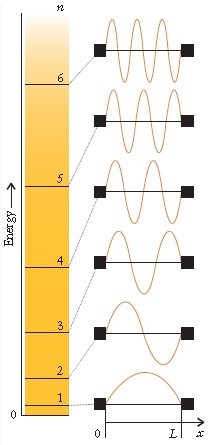
\includegraphics[width=0.25\textwidth]{images/figura1.png}
      \label{fig1}
    \end{figure}

    \par Como $n \in \Re\setminus 0$, a equação \eqref{schrodinger_11} mostra que somente alguns valores para energia são aceitos no confinamento dentro de uma caixa de tamanho L. A partir disso, conclui-se que os níveis de energia de uma partícula confinada são discretos e que a energia pode ser quantizada\cite{frustrado2}.















    